\begin{figure}[htbp]
\centering
\begin{minipage}[t]{0.47\textwidth}
\centering
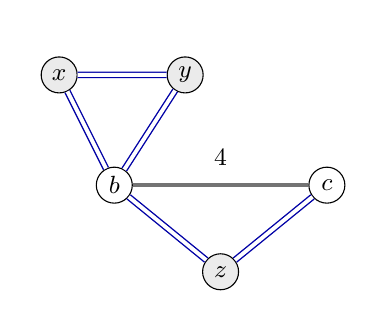
\begin{tikzpicture}[
  vertex/.style={circle,draw,fill=white,minimum size=13pt,inner sep=1pt},
  removed/.style={vertex,fill=black!8},
  doubled/.style={draw=blue!65!black,line width=0.5pt,
                  double=white,double distance=1.4pt},
  bundled/.style={draw=black!55,line width=1.4pt},
  every node/.style={font=\small}]
\node[vertex] (b) at (0,0) {$b$};
\node[removed] (x) at (-0.7,1.4) {$x$};
\node[removed] (y) at (0.9,1.4) {$y$};
\node[vertex] (c) at (2.7,0) {$c$};
\node[removed] (z) at (1.35,-1.1) {$z$};
\draw[doubled] (b) -- (x) -- (y) -- (b);
\draw[doubled] (b) -- (z) -- (c);
\draw[bundled] (b) -- node[above=3pt,text=black] {$4$} (c);
\path[use as bounding box] (-1.1,-1.5) rectangle (3.1,2.0);
\end{tikzpicture}

\small (a) Before suppression
\end{minipage}\hfill
\begin{minipage}[t]{0.50\textwidth}
\centering
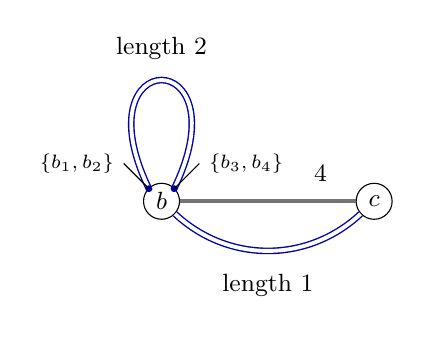
\begin{tikzpicture}[
  vertex/.style={circle,draw,fill=white,minimum size=13pt,inner sep=1pt},
  doubled/.style={draw=blue!65!black,line width=0.5pt,
                  double=white,double distance=1.4pt},
  bundled/.style={draw=black!55,line width=1.4pt},
  every node/.style={font=\small}]
\node[vertex] (b) at (0,0) {$b$};
\node[vertex] (c) at (2.7,0) {$c$};
\coordinate (leftport) at (-0.16,0.16);
\coordinate (rightport) at (0.16,0.16);
\draw[doubled] (leftport)
  .. controls (-1.05,2.0) and (1.05,2.0) ..
  node[pos=0.5,above=4pt] {length $2$} (rightport);
\draw[doubled] (b) to[bend right=43]
  node[midway,below=5pt] {length $1$} (c);
\draw[bundled] (b) -- node[pos=0.8,above=3pt,text=black] {$4$} (c);
\fill[blue!65!black] (leftport) circle (1.25pt);
\fill[blue!65!black] (rightport) circle (1.25pt);
\draw[thin] (leftport) -- (-0.48,0.48)
  node[anchor=east,font=\scriptsize] {$\{b_1,b_2\}$};
\draw[thin] (rightport) -- (0.48,0.48)
  node[anchor=west,font=\scriptsize] {$\{b_3,b_4\}$};
\path[use as bounding box] (-1.7,-1.5) rectangle (3.1,2.0);
\end{tikzpicture}

\small (b) After suppression
\end{minipage}
\caption{The graph of \eqref{eq:encoding-example-word} and its contraction.
Each blue double stroke represents two parallel edge occurrences;
each gray segment labeled $4$ represents four direct $b$--$c$ edges.
Suppressing $x,y$ gives the returning link of length two, with its two
ports marked at $b$. Suppressing $z$ gives the parallel link of length one.
Lengths count removed internal vertices.}
\label{fig:p7-contraction}
\end{figure}
